% vim: set foldmethod=marker foldlevel=0:

\documentclass[a4paper]{article}
\usepackage[UKenglish]{babel}

\usepackage{preamble}

\usepackage{graphicx}
\graphicspath{ {./imgs/} }

\fancyhead[L]{MA146 Assignment 3}
\title{MA146 Methods of Mathematical Modelling 1, Assignment 3}
\colorlet{questionbodycolor}{green!50!teal!50}

\begin{document}

\maketitle

\setlength{\parindent}{0em}
\setlength{\parskip}{1em}

% {{{ Q1
\question{1}

\begin{questionbody}
Objects moving in air experience a drag. Let us specifically consider a ball of radius $r$ that moves with velocity $v$. We assume that its drag $d$ also depends on the density $\rho$ of the air and its dynamic viscosity $\mu$, and write the problem in the form \[
d = u(r, v, \rho, \mu)
\] with some function $u$ that we want to learn more about.

Perform a dimensional analysis using the power of $\mu$ to express the solution to the emerging system of linear equations.

Hint: the viscosity has dimension $[\mu] = M L^{-1} T^{-1}$, and the drag (force) $[d] = M L T^{-2}$
\end{questionbody}

Let $a, b, c, d \in \mathbb Z$. Then \[ [d] = \left[ r^a v^b \rho^c \mu^d \right] = L^a L^b T^{-2b} M^c L^{-3c} M^d L^{-d} T^{-d} = MLT^{-2} \]

Then we get the simultaneous equations \begin{align*}
    c + d &= 1 \\
    a + b - 3c - d &= 1 \\
    -2b - d &= -2
\end{align*}

We don't have enough information to solve the system from here, but we can simplify to get \begin{align*}
    a &= 3 - \frac32 d \\
    b &= 1 - \frac d2 \\
    c &= 1 - d
\end{align*}

Since they're all integers, we know that $d$ is even, so we can just try even values of $d$.

$d=2$ gives \begin{align*}
    a &= 0 \\
    b &= 0 \\
    c &= -1 \\
    d &= 2
\end{align*}
But we want the radius and velocity to be part of the equation, so we don't want $a=b=0$.

$d=4$ gives \begin{align*}
    a &= -3 \\
    b &= -1 \\
    c &= -3 \\
    d &= 4
\end{align*}

Therefore $[d] = \left[ r^{-3} v^{-1} \rho^{-3} \mu^4 \right]$.
% }}}

% {{{ Q2
\newquestion{2}

\begin{questionbody}
To model the freezing of a pond at very cold temperatures, assume that the thickness of the ice on it increases at a rate inversely proportional to its thickness (we here ignore the finite depth of the pond).
\end{questionbody}

\subsection{~} % 2.a

\begin{questionbody}
Denoting the thickness of the ice by $x(t)$ as a function of time $t$, formulate the problem as a differential equation for $x$ using a proportionality constant denoted by $\alpha$.
\end{questionbody}

\[ \dot x(t) = \frac{\alpha}{x(t)} \]

\subsection{~} % 2.b

\begin{questionbody}
If the ice initially (at midnight) is 2mm thick and at 4am it is 3mm thick, how thick will it be at 9:36am?
\end{questionbody}

Let midnight be time $t = 0$, $t$ be in hours and $x(t)$ be in millimetres. Then $x(0) = 2$ and $x(4) = 3$.

\begin{align*}
    \frac{\mathrm d x}{\mathrm d t} &= \frac{\alpha}{x} \\
    \int x \mathrm d x              &= \int \alpha \mathrm d t \\
    \frac{x^2}{2}                   &= \alpha t + C \\
    \therefore x(t)                 &= \sqrt{2\alpha t + C}
\end{align*}

Then we can use the initial values.

\begin{align*}
    x(0) &= \sqrt{2 \alpha \times 0 + C} \\
         &= \sqrt C \\
         &= 2 \\
    \implies C &= 4
\end{align*}

\begin{align*}
    x(2) &= \sqrt{2 \alpha \times 4 + 4} \\
         &= 3 \\
    \implies 8 \alpha &= 3^2 - 4 \\
                      &= 5 \\
    \implies \alpha &= \frac58 \\
    \therefore x(t) &= \sqrt{\frac54 t + 4}
\end{align*}

Now we can just plug in 9:36 am, which is $9.6$ hours after midnight, and find that $x(9.6) = \sqrt{12 + 4} = 4$. Therefore the ice will be 4 mm thick at 9:36 am.

\subsection{~} % 2.c

\begin{questionbody}
Assume that the proportionality factor $\alpha$ is replaced by a time dependent function of the form $\alpha(1 + \cos(\omega t))$, which aims for modelling temperature changes during the day. Here, $t$ is time measured in hours (denoted $h$) and $\omega = \f{2\pi}{24h}$.

Assuming also an initial condition of the form $x(t_0) = x_0$, find the ice thickness as a function of time. (You may keep the parameter $\alpha$, no need to replace it with the value from part \textbf{(b)}.)
\end{questionbody}

Now we have the differential equation \[ \dot x(t) = \frac{\alpha \left(1 + \cos\left( \frac{\pi}{12} t \right)\right)}{x(t)} \]

We can solve this like before, \begin{align*}
    \frac{\mathrm d x}{\mathrm d t} &= \frac{\alpha \left(1 + \cos\left( \frac{\pi}{12} t \right)\right)}{x} \\[1ex]
    \int x \mathrm d x &= \int \alpha \left( 1 + \cos\left(\frac{\pi}{12} t\right) \right) \mathrm d t \\[1ex]
    \frac{x^2}{2} &= \alpha t + \alpha \frac{12}{\pi} \sin \left(\frac{\pi}{12} t\right) + C \\[1ex]
    \therefore x(t) &= \sqrt{2\alpha t + \frac{24\alpha}{\pi} \sin \left(\frac{\pi}{12} t\right) + C}
\end{align*}

Let $t_0 = 0$. Then $x(t_0) = x(0) = \sqrt{0 + \frac{24 \alpha}{\pi} \sin 0 + C} = \sqrt{C} = x_0$, therefore $C = {(x_0)}^2$.

Therefore, \[ x(t) = \sqrt{2\alpha t + \frac{24\alpha}{\pi} \sin \left(\frac{\pi}{12} t\right) + {(x_0)}^2} \]
% }}}

% {{{ Q3
\newquestion{3}

\begin{questionbody}
A model for the vibrations of a wine glass is given by the differential equation \begin{equation}\label{eqn:Q3-vibrations-ode}
x''(t) + \lambda x'(t) + \omega^2 x(t) = f(t)
\end{equation}
where $x$ is some measure of the deformation, $\lambda, \omega > 0$ are given numbers and $f$ is a given function called \textit{(acoustic) forcing}. The equation is nondimensional. The glass shatters if $|x(t)| \ge 1$ at any time $t$.

Please get the Jupyter notebook \texttt{MA146\_Assignment3.ipynb} for this question. It contains an example on how to solve initial value problems for second order equations with \texttt{sympy}.
\end{questionbody}

\subsection{~} % 3.a

\begin{questionbody}
Use the notebook to symbolically solve the initial value problem \[
x''(t) + \lambda x'(t) + \omega^2 x(t) = 0, \quad x(0) = x_i, x'(0) = d_i
\] with $\lambda = 0.8$, $\omega = 5.0$, $x_i = 0$, and $d_λ = 3.6$.

Provide your code, the algebraic expression for the solution produced by the software, and a plot on the interval $(0, 3\pi)$ for $t$ of the solution.
\end{questionbody}

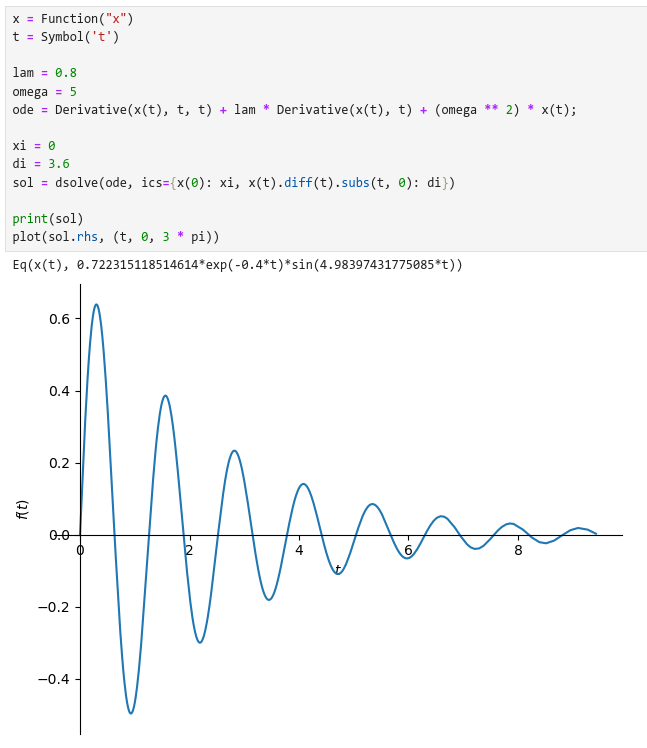
\includegraphics[scale=0.6]{Q3-a}

\subsection{~} % 3.b

\begin{questionbody}
Implement now a solver for~\eqref{eqn:Q3-vibrations-ode} with \[
f(t) = a \cos(\alpha t)
\] and initial conditions \[
x(0) = 0, x'(0) = 0.
\] Assume that the parameters are $\lambda = 0.0009$, $\omega = 6.415$, $\alpha = 2\pi$.

Use your solver to computationally (for instance, by try and error) find the smallest number $n \in \N$ such that $a = n/10$ is sufficient to ensure that $x(t) \ge 1$ at some time $t$ (i.e., the factor in the forcing is big enough to break the glass).

Provide your solution ($n$ and $a$) and, for evidence, two graphs, one for the minimal $n_\text{min}$ and one for $n_\text{min} - 1$.

(Hints: Start with $n = 3$. You will need a sufficiently large domain for $t$ to see what is going on, for instance, $t \in (0, 60)$.

You might observe some odd behaviour in the graph but which (hopefully) are visualisation effects only. They should vanish if you increase the number of points in the variable \texttt{nb\_of\_points} that is used in the plotting command.)
\end{questionbody}

My solution is $n_\text{min} = 9$.

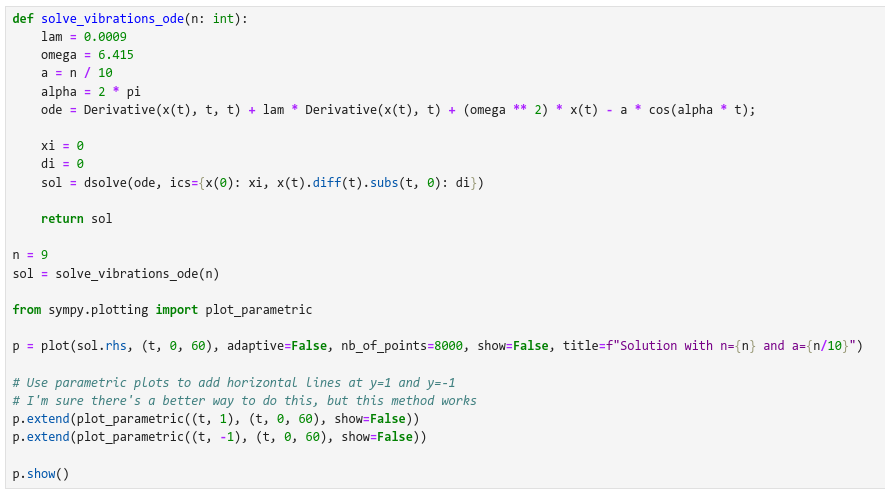
\includegraphics[width=\linewidth]{Q3-b}
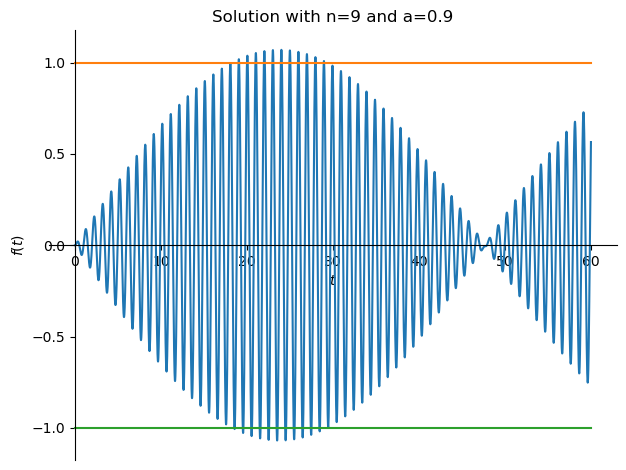
\includegraphics[width=\linewidth]{n9}
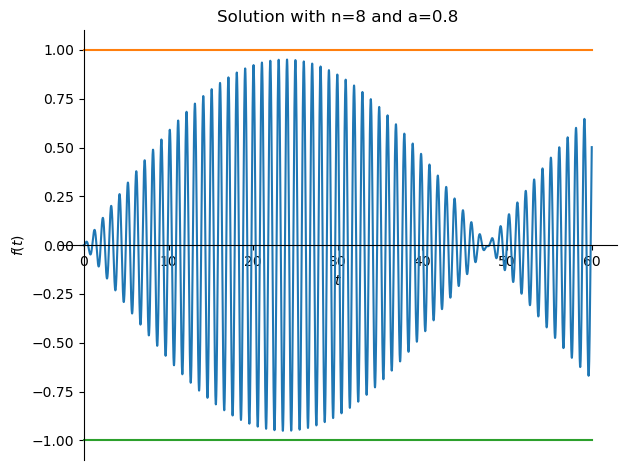
\includegraphics[width=\linewidth]{n8}
% }}}

% {{{ Q4
\newquestion{4}

\begin{questionbody}
Find a particular integral for the second order differential equation \[
\ddd 2{} y(t) + \eta \diff t y(t) + b y(t) = f \cos (\theta t)
\] with parameters $b, \eta, \theta, f > 0$.
\end{questionbody}

Since the right hand side is $f \cos(\theta t)$, we will use $y(t) = A \cos(\theta t) + B \sin(\theta t)$ as our particular integral.
\begin{align*}
    y(t)   &= A \cos(\theta t) + B \sin(\theta t) \\
    y'(t)  &= -\theta A \sin(\theta t) + \theta B \cos(\theta t) \\
    y''(t) &= -\theta^2 A \cos(\theta t) - \theta^2 B \sin(\theta t)
\end{align*}

Plugging this into the ODE, we get \[
-\theta^2 A \cos(\theta t) - \theta^2 B \sin(\theta t) -\eta\theta A \sin(\theta t) + \eta\theta B \cos(\theta t) + bA \cos(\theta t) + bB \sin(\theta t) = f \cos(\theta t)
\]

We can compare coefficients of $\sin$ and $\cos$ and conclude that \begin{align*}
    -\theta^2 B - \eta\theta A + bB &= 0 \\
    -\theta^2 A - \eta\theta B + bA &= f
\end{align*}

The first equation implies $B(b - \theta^2) = \eta\theta A$. We can use this to get $B$ in terms of $A$, so $B = \dfrac{\eta\theta A}{b - \theta^2}$. Then we can plug that into the second equation, which gives \[
A \left(-\theta^2 + \frac{\eta^2 \theta^2}{b - \theta^2} + b\right) = f
\]

Therefore \[ A = \frac{f (b - \theta^2)}{{(b - \theta^2)}^2 + \eta^2 \theta^2} \]

And therefore \[ B = \frac{\eta \theta f}{{(b - \theta^2)}^2 + \eta^2 \theta^2} \]

Therefore the particular integral is \[
\frac{f (b - \theta^2)}{{(b - \theta^2)}^2 + \eta^2 \theta^2} \cos(\theta t) + \frac{\eta \theta f}{{(b - \theta^2)}^2 + \eta^2 \theta^2} \sin (\theta t)
\]

Alternatively written as \[
\frac{f}{{(b - \theta^2)}^2 + \eta^2 \theta^2} \left( (b - \theta^2) \cos(\theta t) + \eta \theta \sin(\theta t) \right)
\]
% }}}

\end{document}
